\documentclass[devoir3.tex]{subfiles}

\begin{document}

\section*{Question 4}
Supposez que vous ayez un damier \(n \times n\) et un jeton. Vous devez déplacer
le jeton depuis le bord inferieur du damier vers le bord supérieur, en respectant la règle suivante. À chaque étape, vous pouvez placer le jeton sur l’un des trois carrés suivants

\begin{itemize}
	\item le carré qui est juste au dessus,
	\item le carré qui est une position plus haut et une position plus à gauche (à condition que le jeton ne soit pas déjà dans la colonne la plus à gauche),
	\item le carré qui est une position plus haut et une position plus à droite (à condition que le jeton ne soit pas déjà dans la colonne la plus à droite).
\end{itemize}

\begin{figure}[H]
	\centering
	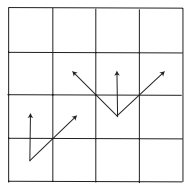
\includegraphics[width=6cm]{fig2}
	\caption{Graphe}
	\label{fig:fig2}
\end{figure}

La figure \ref{fig:fig2} illustre les déplacements valides à partir de deux positions dans un damier de dimension \(4 \times 4\). \\

Chaque fois que vous vous déplacez du carré \(x = (i, j)\) au carré \(y \in \lbrace (i-1,j-1),(i-1,j),(i-1,j+1) \rbrace \), vous recevez \(p(x, y)\) dollars. On vous donne \(p(x, y)\) pour toutes les paires \((x, y)\) correspondant à un déplacement licite de \(x\) à \(y\). \(p(x, y)\) \textbf{n’est pas forcément positif}. \\

Donner un algorithme efficace de programmation dynamique pour déterminer le montant maximum que vous pouvez empocher. Votre algorithme peut partir de n’importe quel carré du bord inférieur et arriver sur n’importe quel carré du bord supérieur pour maximiser le montant collecté au cours du trajet. \\

Expliquez comment vous pouvez optimiser l’espace mémoire et évaluez le temps d’exécution et l’espace mémoire de votre algorithme. \\

\newpage

Il est possible de facilement constater que ce problème de programmation dynamique présente une structure caractéristique qui le prête bien à ce genre d'algorithme. En effet, la résolution de ce problème se fait en résolvant les sous-problèmes.\\

Pour comprendre comment résoudre les sous-problèmes, il suffit de comprendre que, pour obtenir le meilleur résultat, nous n'avons qu'à partir de la fin du problème (du rang n jusqu'au rang 1) et de récursivement descendre en trouvant la case précédente qui nous génère le plus grand montant. Ensuite, nous n'avons qu'à refaire cela pour chaque case final et ainsi obtenir le chemin le plus payant.\\

Voici un démonstatration rapide de cet algorithme en utilisant une gille 6x6.\\

\begin{tikzpicture}[scale=1.50]
\foreach \x in {1, 2, ..., 6}
\foreach \y in {1, 2, ..., 6}
{
	\draw (\x,\y) +(-.5, -.5) rectangle ++(.5, .5);
}
\foreach \x in {1, 2, ..., 6}
{
	\node at (\x, 0) {\x};
	\node at (0, \x) {\x};
}
\draw (3, 4) node{\small A};
\draw (2, 3) node{\small B};
\draw (3, 3) node{\small C};
\draw (4, 3) node{\small D};
\end{tikzpicture}

Pour choisir le bon chemin à partir de A, il suffit de choisir la valeur la plus élevée de la fonction \( P \) entre B, C ou D. On construit donc la valeur de \( P \) pour le point A à partir des valeurs inférieure.

On obtient donc l'équations suivante:

\[ P(A) = max(P(B), P(C), P(D)) + C(A)) \]

où \( C \) est une fonction qui calcule le coût de l'emplacement.\\

Il est possible aussi de se rendre compte que si le jeton est sur les côtés, la valeur du du côté gauche du jeton (s'il est du côté gauche) doit être de -infini pour que celui-ci ne choisisse pas ce chemin. Il est donc possible de facilement définir un algorithme en pseudo-code pour réaliser ceci.\\

\begin{algorithm}[H]
	\KwData{\( P[1 \dots n,1 \dots n] \: entier \: i, entier \: j \)}
    \KwResult{\(valeur \: de \: i, \: j\)}

    \If{ \( j < 1 \: ou \: j > n \) }{
    	\Return \( -infini \)
    }

		\ElseIf{ \( i = 1 \) }{
    	\Return \( C(i, \: j) \)
    }

		\Else{
    	\Return \( max(F(i \: - \: 1, \: j \: - \: 1), \: F(i \: - \: 1, \: j), \: F(i \: - \: 1, \: j \: + \: 1)) \: + \: C(i, \: j) \)
    }

      \caption{Fonction F: Trouver le chemin le plus payant}
\end{algorithm}

Il est possible d'analyser cet algorithme:\\

Pour la complexité temporelle, on voit extrêmement facilement que pour chaque boucle récursive, on descend d'un rang. Puisque l'on descend d'un rang à chaque fois, et qu'il y a \( n \) rang, et que dans chaque boucle, choisir la prochaine étape ce fait en \( O(3) \) (d'ou \( O(1) \)).\\

Il est possible de conclure que la notation grand O de cet algorithme est de \( O(n \: * \: 1) \: = \: O(n) \).\\

Pour la complexité spatiale, on voit également facilement que cet algorithme utilise seulement un tableau de \(n\) par \(n\). On voit donc que la complexité spatiale est de \(O(n^2)\).\\

Il serait possible d'optimiser cet algorithme en conservant la valeur de C entre chaque exécution. L'avantage de cela serait de ne pas recalculer pour chaque fois que l'on veut la valeur maximale d'une nouvelle case. On pourrait également remplacer le tableau en une simple liste, chaînée ou non, si l'on veut que contenir le chemin et sa valeur jusqu'à maintenant. Cela diminue la complexité spatiale du problème.

\end{document}
